% Options for packages loaded elsewhere
\PassOptionsToPackage{unicode}{hyperref}
\PassOptionsToPackage{hyphens}{url}
\PassOptionsToPackage{dvipsnames,svgnames,x11names}{xcolor}
%
\documentclass[
  letterpaper,
  DIV=11,
  numbers=noendperiod]{scrartcl}

\usepackage{amsmath,amssymb}
\usepackage{iftex}
\ifPDFTeX
  \usepackage[T1]{fontenc}
  \usepackage[utf8]{inputenc}
  \usepackage{textcomp} % provide euro and other symbols
\else % if luatex or xetex
  \usepackage{unicode-math}
  \defaultfontfeatures{Scale=MatchLowercase}
  \defaultfontfeatures[\rmfamily]{Ligatures=TeX,Scale=1}
\fi
\usepackage{lmodern}
\ifPDFTeX\else  
    % xetex/luatex font selection
\fi
% Use upquote if available, for straight quotes in verbatim environments
\IfFileExists{upquote.sty}{\usepackage{upquote}}{}
\IfFileExists{microtype.sty}{% use microtype if available
  \usepackage[]{microtype}
  \UseMicrotypeSet[protrusion]{basicmath} % disable protrusion for tt fonts
}{}
\makeatletter
\@ifundefined{KOMAClassName}{% if non-KOMA class
  \IfFileExists{parskip.sty}{%
    \usepackage{parskip}
  }{% else
    \setlength{\parindent}{0pt}
    \setlength{\parskip}{6pt plus 2pt minus 1pt}}
}{% if KOMA class
  \KOMAoptions{parskip=half}}
\makeatother
\usepackage{xcolor}
\setlength{\emergencystretch}{3em} % prevent overfull lines
\setcounter{secnumdepth}{-\maxdimen} % remove section numbering
% Make \paragraph and \subparagraph free-standing
\makeatletter
\ifx\paragraph\undefined\else
  \let\oldparagraph\paragraph
  \renewcommand{\paragraph}{
    \@ifstar
      \xxxParagraphStar
      \xxxParagraphNoStar
  }
  \newcommand{\xxxParagraphStar}[1]{\oldparagraph*{#1}\mbox{}}
  \newcommand{\xxxParagraphNoStar}[1]{\oldparagraph{#1}\mbox{}}
\fi
\ifx\subparagraph\undefined\else
  \let\oldsubparagraph\subparagraph
  \renewcommand{\subparagraph}{
    \@ifstar
      \xxxSubParagraphStar
      \xxxSubParagraphNoStar
  }
  \newcommand{\xxxSubParagraphStar}[1]{\oldsubparagraph*{#1}\mbox{}}
  \newcommand{\xxxSubParagraphNoStar}[1]{\oldsubparagraph{#1}\mbox{}}
\fi
\makeatother


\providecommand{\tightlist}{%
  \setlength{\itemsep}{0pt}\setlength{\parskip}{0pt}}\usepackage{longtable,booktabs,array}
\usepackage{calc} % for calculating minipage widths
% Correct order of tables after \paragraph or \subparagraph
\usepackage{etoolbox}
\makeatletter
\patchcmd\longtable{\par}{\if@noskipsec\mbox{}\fi\par}{}{}
\makeatother
% Allow footnotes in longtable head/foot
\IfFileExists{footnotehyper.sty}{\usepackage{footnotehyper}}{\usepackage{footnote}}
\makesavenoteenv{longtable}
\usepackage{graphicx}
\makeatletter
\def\maxwidth{\ifdim\Gin@nat@width>\linewidth\linewidth\else\Gin@nat@width\fi}
\def\maxheight{\ifdim\Gin@nat@height>\textheight\textheight\else\Gin@nat@height\fi}
\makeatother
% Scale images if necessary, so that they will not overflow the page
% margins by default, and it is still possible to overwrite the defaults
% using explicit options in \includegraphics[width, height, ...]{}
\setkeys{Gin}{width=\maxwidth,height=\maxheight,keepaspectratio}
% Set default figure placement to htbp
\makeatletter
\def\fps@figure{htbp}
\makeatother

\KOMAoption{captions}{tableheading}
\makeatletter
\@ifpackageloaded{caption}{}{\usepackage{caption}}
\AtBeginDocument{%
\ifdefined\contentsname
  \renewcommand*\contentsname{Table of contents}
\else
  \newcommand\contentsname{Table of contents}
\fi
\ifdefined\listfigurename
  \renewcommand*\listfigurename{List of Figures}
\else
  \newcommand\listfigurename{List of Figures}
\fi
\ifdefined\listtablename
  \renewcommand*\listtablename{List of Tables}
\else
  \newcommand\listtablename{List of Tables}
\fi
\ifdefined\figurename
  \renewcommand*\figurename{Figure}
\else
  \newcommand\figurename{Figure}
\fi
\ifdefined\tablename
  \renewcommand*\tablename{Table}
\else
  \newcommand\tablename{Table}
\fi
}
\@ifpackageloaded{float}{}{\usepackage{float}}
\floatstyle{ruled}
\@ifundefined{c@chapter}{\newfloat{codelisting}{h}{lop}}{\newfloat{codelisting}{h}{lop}[chapter]}
\floatname{codelisting}{Listing}
\newcommand*\listoflistings{\listof{codelisting}{List of Listings}}
\makeatother
\makeatletter
\makeatother
\makeatletter
\@ifpackageloaded{caption}{}{\usepackage{caption}}
\@ifpackageloaded{subcaption}{}{\usepackage{subcaption}}
\makeatother

\ifLuaTeX
  \usepackage{selnolig}  % disable illegal ligatures
\fi
\usepackage{bookmark}

\IfFileExists{xurl.sty}{\usepackage{xurl}}{} % add URL line breaks if available
\urlstyle{same} % disable monospaced font for URLs
\hypersetup{
  pdftitle={Hazard Identification},
  pdfauthor={Zheng Zhou},
  colorlinks=true,
  linkcolor={blue},
  filecolor={Maroon},
  citecolor={Blue},
  urlcolor={Blue},
  pdfcreator={LaTeX via pandoc}}


\title{Hazard Identification}
\author{Zheng Zhou}
\date{2025-09-12}

\begin{document}
\maketitle


\subsection{Introduction}\label{introduction}

\begin{itemize}
\tightlist
\item
  Risk = Hazard * Exposure
\end{itemize}

\begin{figure}[H]

{\centering 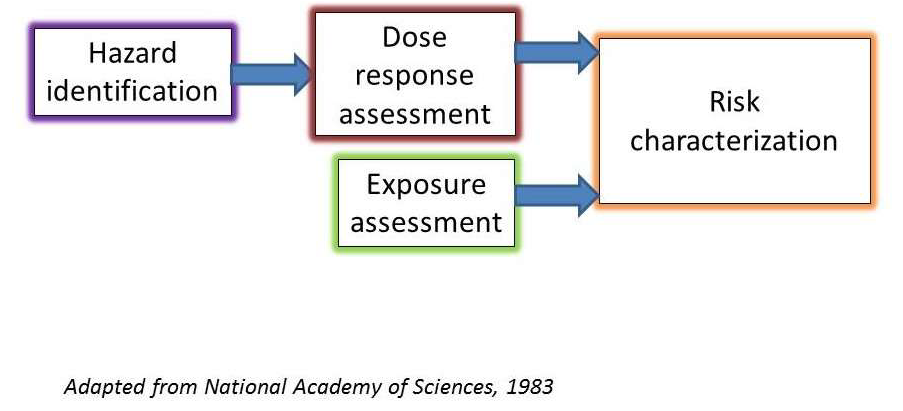
\includegraphics{risk_paradigm.png}

}

\caption{Risk Assessment Paradigm}

\end{figure}%

\subsection{Hazard Identification and
Characterization}\label{hazard-identification-and-characterization}

Different questions of interest:

\begin{itemize}
\item
  Identification: YES/NO
\item
  Characterization: dose-response models
\end{itemize}

\subsection{Validity: Hierarchy of
Evidence}\label{validity-hierarchy-of-evidence}

\begin{figure}[H]

{\centering 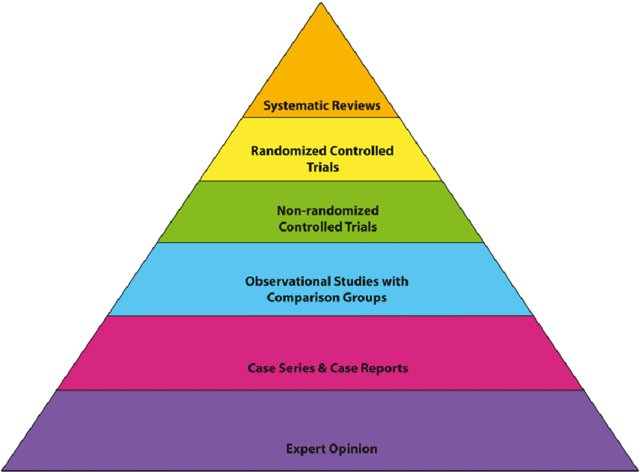
\includegraphics{Evidence_pyramid.png}

}

\caption{Evidence Pyramid (Golden and Bass 2013)}

\end{figure}%

\subsubsection{Opinion without evidence}\label{opinion-without-evidence}

\begin{itemize}
\item
  \textbf{NOT} expert judgement; \textbf{Not necessarily} from experts
\item
  Strength: useful in the lack of empirical evidence
\item
  Weakness: low validity (not necessarily wrong!)
\end{itemize}

\subsubsection{Case report \& case
series}\label{case-report-case-series}

\begin{itemize}
\item
  Definition
\item
  Strength: simple in design and practice
\item
  Weakness: no account for bias; generalizability
\end{itemize}

\subsubsection{Observational studies}\label{observational-studies}

\begin{itemize}
\item
  Definition: observational vs interventional
\item
  Type: case control, cohort
\item
  Strength: generalizable within study groups; less bias from comparison
\item
  Weakness: no full account for bias
\end{itemize}

\subsubsection{Controlled experiments (randomized and
non-randomized)}\label{controlled-experiments-randomized-and-non-randomized}

\begin{itemize}
\item
  Definition: direct intervention; group assignment
\item
  Strength: direct evaluation of impact of intervention to reduce bias
\item
  Weakness: time-consuming, expensive, ethical challenges
\end{itemize}

\subsubsection{Systematic reviews}\label{systematic-reviews}

\begin{itemize}
\item
  Strength: consider existing evidence for their results, validity and
  generalizability; adaptive
\item
  Weakness: complicated and affected by review methodology
\end{itemize}

\subsection{Type: Lines of Empirical
Evidence}\label{type-lines-of-empirical-evidence}

Type: human, animal (in vivo), non-animal (in vitro, new-approach
methodologies)

\subsubsection{Human Experiments}\label{human-experiments}

Atrocities within sight:

\begin{itemize}
\item
  during WWI, deliberate and pseudo-scientific experiments and torture
  on human by Japanese and German Nazi
\item
  Tuskegee Syphilis study (1932-1972) by US government, targeting
  African Americans
\end{itemize}

\subsubsection{Why we don't conduct human
experiments}\label{why-we-dont-conduct-human-experiments}

\begin{itemize}
\tightlist
\item
  Ethics: ``\emph{Cannot deliberately expose humans to potentially
  harmful agents.}''
\end{itemize}

Watch the videos on:

\href{https://youtu.be/_oZAPk_Xpow?si=XIJO6INIEd5m6HqC}{The Nuremberg
Code (1947)}

\href{https://youtu.be/dFmI3wNzL8k?si=A5ROtryw-QfJehx3}{Declaration of
Helsinki (1964) by the World Medical Association}

\href{https://youtu.be/M6AKIIhoFn4?si=L35kK5pfyzD-bO-t}{The Belmont
Report (1979) after the Tuskegee experiment}

Mandate on Institutional Review Boards(US); Swedish Ethical Review
Authority (Etikprövningsmyndigheten)

\begin{itemize}
\item
  Potential harmful agents: observational evidence in human + controlled
  experiments in animal and non-animal systems
\item
  Beneficial agents: controlled trails, voluntary participation after
  complete transparency
\end{itemize}

\subsubsection{Epidemiological studies}\label{epidemiological-studies}

\begin{itemize}
\item
  Definition: Observational studies on human
\item
  Design: prospective vs retrospective, sampling, extrapolation
\item
  Limitations in interpretation: results from epidemiological studies
  should only be interpreted as associations, not causations
\end{itemize}

\subsubsection{Animal studies}\label{animal-studies}

\begin{itemize}
\item
  Species: rodents (rats, mice), fish, earthworm, dogs, monkeys, etc.
\item
  Strength: free from human ethical concerns; precise controls;
  mechanistic insights
\item
  Weakness: intra-species difference

  \begin{itemize}
  \item
    More toxic to animal than human: DDT (Silent Spring by Rachel
    Carson, 1962)
  \item
    More toxic to human than animal: arsenic
    (\href{https://www.who.int/news-room/fact-sheets/detail/arsenic}{WHO
    arsenic facts})
  \item
    Acute animal dosing for chronic human exposure
  \end{itemize}
\end{itemize}

\subsubsection{Non-animal studies}\label{non-animal-studies}

\begin{itemize}
\item
  Type: in vitro (cell/tissue cultures), in silico (computational
  modeling/simulations)
\item
  Example: physiologically-based artificial organ system, human cell
  genome analysis (omics), quantitative structure-activity relationship
  models
\item
  Strength: free of animal use
  (\href{https://ki.se/en/research/popular-science-and-dialogue/animal-research/the-principles-of-3r}{3R
  principles})- rapid, high-throughput, cost-effective, no ethical
  concerns
\item
  Weakness: still developing, limited acceptance in regulation and
  application
\end{itemize}

\subsection{Discussion and Exercise}\label{discussion-and-exercise}

Separate into two groups and discussion the following questions (5 min):

\begin{enumerate}
\def\labelenumi{\arabic{enumi}.}
\item
  considering the strength and weakness of each line of evidence, how
  they compliment each other.
\item
  fill in the following table: intersection between type and validity of
  evidence
\end{enumerate}

\begin{longtable}[]{@{}
  >{\raggedright\arraybackslash}p{(\columnwidth - 8\tabcolsep) * \real{0.2000}}
  >{\raggedright\arraybackslash}p{(\columnwidth - 8\tabcolsep) * \real{0.2000}}
  >{\raggedright\arraybackslash}p{(\columnwidth - 8\tabcolsep) * \real{0.2000}}
  >{\raggedright\arraybackslash}p{(\columnwidth - 8\tabcolsep) * \real{0.2000}}
  >{\raggedright\arraybackslash}p{(\columnwidth - 8\tabcolsep) * \real{0.2000}}@{}}
\toprule\noalign{}
\begin{minipage}[b]{\linewidth}\raggedright
Evidence type
\end{minipage} & \begin{minipage}[b]{\linewidth}\raggedright
Case report \& series
\end{minipage} & \begin{minipage}[b]{\linewidth}\raggedright
Observational studies
\end{minipage} & \begin{minipage}[b]{\linewidth}\raggedright
Controlled trails
\end{minipage} & \begin{minipage}[b]{\linewidth}\raggedright
Systematic Reviews
\end{minipage} \\
\midrule\noalign{}
\endhead
\bottomrule\noalign{}
\endlastfoot
Human experiment & \ldots{} & \ldots{} & \ldots{} & \ldots{} \\
Epidemiological studies & \ldots{} & \ldots{} & \ldots{} & \ldots{} \\
Animal studies & \ldots{} & \ldots{} & \ldots{} & \ldots{} \\
Non-animal studies & \ldots{} & \ldots{} & \ldots{} & \ldots{} \\
\end{longtable}

\subsection{Causal inference}\label{causal-inference}

Central question: inference for \textbf{causality}

``\emph{Was the hazard \textbf{caused} by the agent of interest?}''

``\emph{Will the intervention \textbf{cause} a reduction in the
hazard?}''

\subsubsection{Correlation is NOT
Causation}\label{correlation-is-not-causation}

Our intuitive inference are based on \textbf{correlation}.

\textbf{Example1}: People who use more sunscreen also have higher rates
of skin cancer

\textbf{Example2}: In the United States, the per capita crime rates are
higher among people of brown and black skin color

\textbf{Example3}: Number of people drown increases when ice cream
consumption increases

Highlights:

\begin{itemize}
\tightlist
\item
  \textbf{Correlation} does not imply a \textbf{causal relationship}.
\item
  Lack of \textbf{correlation} does not imply a lack of \textbf{causal
  relationship}.
\item
  There may be \textbf{biases} that explain the observed association.
\end{itemize}

\subsubsection{Threats to validity in observational and non-randomized
intervention
studies}\label{threats-to-validity-in-observational-and-non-randomized-intervention-studies}

\begin{enumerate}
\def\labelenumi{\arabic{enumi}.}
\tightlist
\item
  \textbf{Selection Bias}: When individuals self-select into treatment
  groups, leading to systematic differences between groups.

  \begin{itemize}
  \tightlist
  \item
    \textbf{Example}: People who opt for an exercise program may already
    be healthier than those who do not.
  \end{itemize}
\item
  \textbf{Confounding}: A third variable affects both the treatment and
  the outcome, leading to biased estimates.

  \begin{itemize}
  \tightlist
  \item
    \textbf{Example}: A new teaching method might be adopted in schools
    that already have higher-performing students.
  \end{itemize}
\item
  \textbf{Maturation}: Changes in subjects occur naturally over time,
  not because of the treatment.

  \begin{itemize}
  \tightlist
  \item
    \textbf{Example}: Children naturally improve in cognitive skills as
    they age, regardless of an educational intervention.
  \end{itemize}
\item
  \textbf{History}: External events occurring during the study may
  affect outcomes.

  \begin{itemize}
  \tightlist
  \item
    \textbf{Example}: An economic crisis affecting income levels during
    a study of financial literacy interventions.
  \end{itemize}
\end{enumerate}

\subsubsection{Observational designs}\label{observational-designs}

\textbf{Simple Comparison}

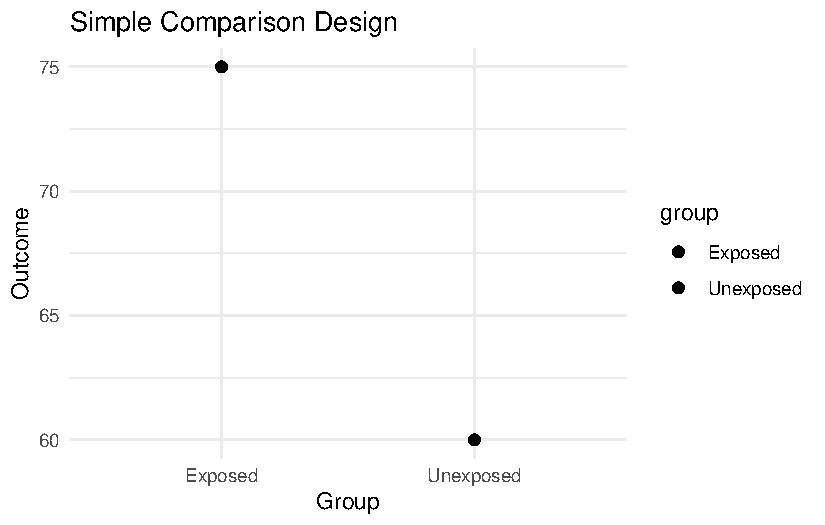
\includegraphics{lecture_hazardID_files/figure-pdf/unnamed-chunk-1-1.pdf}

Easy to implement; Comparison at one time point only.

\textbf{One-group pre-post comparison}

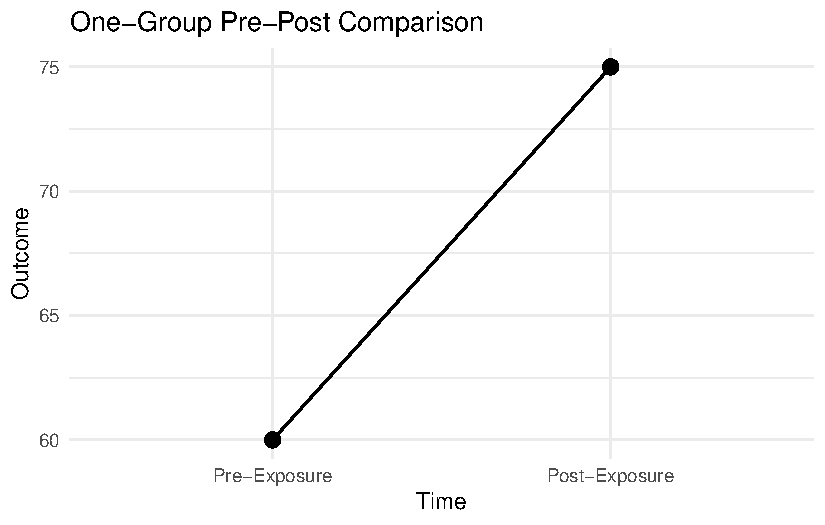
\includegraphics{lecture_hazardID_files/figure-pdf/unnamed-chunk-2-1.pdf}

Check for baseline difference

\textbf{Multi-group pre-post comparisons}

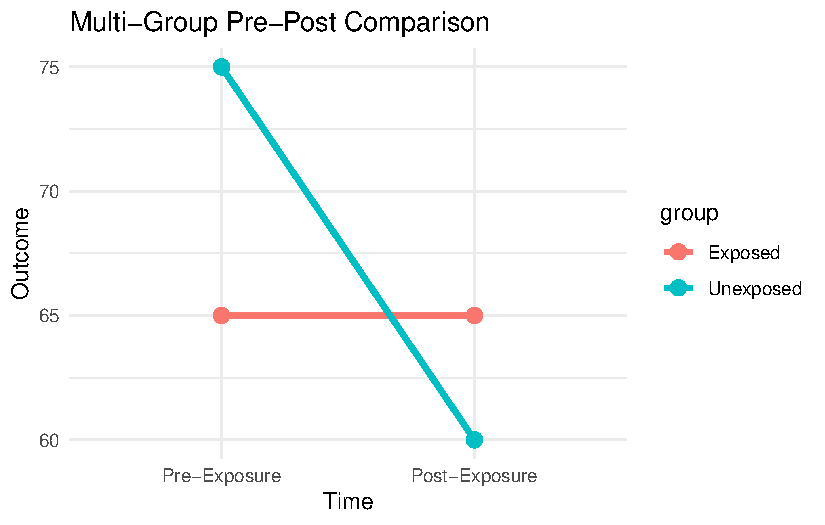
\includegraphics{lecture_hazardID_files/figure-pdf/unnamed-chunk-3-1.pdf}

\subsubsection{Bradford Hill
considerations}\label{bradford-hill-considerations}

By Austin Bradford Hill 1965, causal inference in epidemiological
studies.

Nine considerations:

\begin{itemize}
\item
  Strength
\item
  Consistency
\item
  Specificity
\item
  Temporality: the ONLY necessary condition for causality among the nine
\item
  Biological Gradient
\item
  Plausibility
\item
  Coherence
\item
  Experiment
\item
  Analogy
\end{itemize}

\href{https://research.ebsco.com/c/hrh7jr/viewer/html/4j23s2octz}{Hall,
2024. Austin Bradford Hill's `Environment and disease: Association or
causation'.Addition.}

Hill's considerations:

\begin{itemize}
\item
  Not designed as a definitive criteria, thus should not be used as one
\item
  All Hill's considerations satisifed without causality: ice cream
  consumption and drowning
\end{itemize}

\subsubsection{Counterfacuals}\label{counterfacuals}

Identification question: ``\emph{Was the hazard \textbf{caused} by the
agent of interest?}''

Countefactual: ``Would the \textbf{same individual subject} develop the
same hazard, \emph{if anything else were the same}, without exposure to
the agent of interest?''

``Will hazard on the \textbf{same subject} be reduced, \emph{if anything
else were the same}, without the intervention?''

By comparing the treatment with the counterfactual, these threats are
effectively controlled.

Counterfactuals cannot remove biases, but isolate the causal effect from
biases.

\subsubsection{Randomized Controlled trails as approximations to
counterfactuals}\label{randomized-controlled-trails-as-approximations-to-counterfactuals}

Challenge to counterfactuals: Current human technology has no method to
observe counterfactuals.

Approximation: randomized assignment into intervention and control
groups

RCT question: ``What would happen if everything is the same
\textbf{between groups} except the intervention/exposed?''

Randomized controlled trails is the GOLD STANDARD of causal inference.

\subsubsection{Directions to Advanced Causal
Inference}\label{directions-to-advanced-causal-inference}

Experimental design

\begin{itemize}
\item
  What is the minimal sample size required for randomization?
\item
  What if we want to introduce magnitude of treatment into
  randomization?
\item
  What if the sample needs to be stratified to represent the population?
\item
  Empirical evaluation of observational evidence
\end{itemize}

Quasi-experimental methods (such as instrumental variable)

\begin{itemize}
\item
  What assumption underlines these methods?
\item
  To what extent their conclusion could be generalized?
\end{itemize}

\subsection{Questions?}\label{questions}

Afternoon at 1-3pm at Biosfären (Sal 220)




\end{document}
